% apparatus_schematic.tex - 实验装置与微流控结构示意图模板 (Apparatus Schematic)
% 编译方式: pdflatex apparatus_schematic.tex 或 xelatex apparatus_schematic.tex
\documentclass[tikz,border=10pt]{standalone}
\usepackage{xcolor}
\usepackage{tikz}
\usetikzlibrary{arrows.meta, positioning, calc, shapes.geometric, backgrounds}

\definecolor{natureblue}{HTML}{4E79A7}
\definecolor{natureorange}{HTML}{F28E2B}
\definecolor{naturered}{HTML}{E15759}
\definecolor{naturecyan}{HTML}{76B7B2}
\definecolor{darktext}{HTML}{262626}
\definecolor{subtext}{HTML}{64748B}
\definecolor{chipbg}{HTML}{F8FAFC}
\definecolor{chipborder}{HTML}{CBD5E1}
\definecolor{oilphase}{HTML}{D97706}
\definecolor{waterphase}{HTML}{0284C7}

\begin{document}
\sffamily
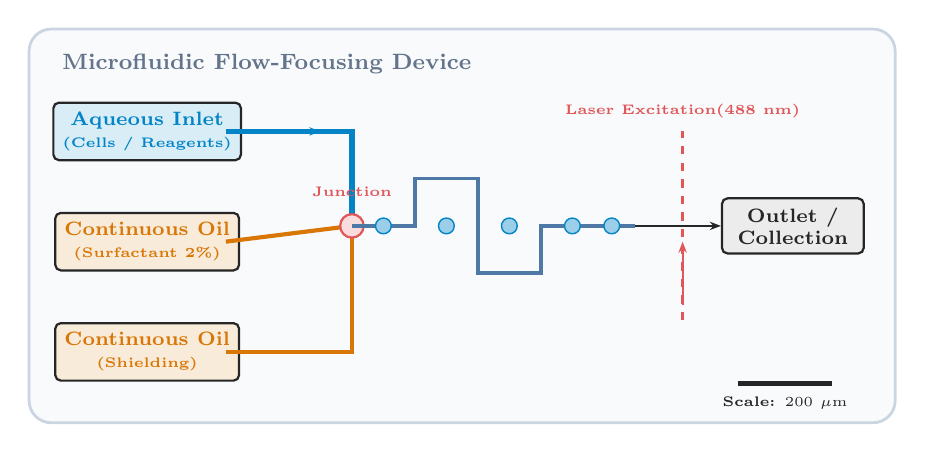
\begin{tikzpicture}[
    scale=1.0,
    port/.style={
        rectangle,
        rounded corners=2pt,
        draw=darktext,
        line width=0.8pt,
        minimum width=1.8cm,
        minimum height=0.65cm,
        align=center,
        font=\scriptsize\bfseries
    },
    flowarrow/.style={
        -{Stealth[length=4pt,width=3pt]},
        line width=0.8pt
    }
]

    % --- 1. 芯片透明基底轮廓 ---
    \draw[fill=chipbg, draw=chipborder, line width=1.0pt, rounded corners=8pt] (-0.5, -0.5) rectangle (10.5, 4.5);
    \node[anchor=north west, font=\footnotesize\bfseries\color{subtext}] at (-0.2, 4.3) {Microfluidic Flow-Focusing Device};

    % --- 2. 进样端口与流体管路 ---
    % 水相进样口 (Aqueous phase)
    \node[port, fill=waterphase!15, text=waterphase] (inlet1) at (1.0, 3.2) {Aqueous Inlet\\{\tiny (Cells / Reagents)}};
    % 油相进样口 1 (连续相顶部)
    \node[port, fill=oilphase!15, text=oilphase] (inlet2) at (1.0, 1.8) {Continuous Oil\\{\tiny (Surfactant 2\%)}};
    % 油相进样口 2 (连续相底部)
    \node[port, fill=oilphase!15, text=oilphase] (inlet3) at (1.0, 0.4) {Continuous Oil\\{\tiny (Shielding)}};

    % --- 3. 微通道几何 (Channels) ---
    % 水相主通道
    \draw[waterphase, line width=2.0pt] (2.0, 3.2) -| (3.6, 2.0);
    \draw[flowarrow, color=waterphase] (2.8, 3.2) -- ++(0.4, 0);

    % 油相主通道 (交汇夹击)
    \draw[oilphase, line width=1.5pt] (2.0, 1.8) -- (3.6, 2.0);
    \draw[oilphase, line width=1.5pt] (2.0, 0.4) -| (3.6, 2.0);

    % 十字交汇液滴生成区 (Flow-focusing junction)
    \node[circle, draw=naturered, fill=naturered!20, line width=0.8pt, inner sep=3pt] (junction) at (3.6, 2.0) {};
    \node[anchor=south, font=\tiny\bfseries\color{naturered}] at (3.6, 2.25) {Junction};

    % 混合与延时蛇形通道 (Serpentine mixing channel)
    \draw[color=natureblue, line width=1.2pt] 
        (3.6, 2.0) -- (4.4, 2.0) 
        -- (4.4, 2.6) -- (5.2, 2.6) 
        -- (5.2, 1.4) -- (6.0, 1.4) 
        -- (6.0, 2.0) -- (7.2, 2.0);

    % 生成的微液滴 (Monodisperse droplets)
    \foreach \x in {4.0, 4.8, 5.6, 6.4, 6.9} {
        \draw[fill=waterphase!40, draw=waterphase, line width=0.5pt] (\x, 2.0) circle (0.10cm);
    }

    % --- 4. 原位光学检测窗口 (Laser interrogation) ---
    \draw[color=naturered, line width=1.0pt, dashed] (7.8, 0.8) -- (7.8, 3.2);
    \node[anchor=south, font=\tiny\bfseries\color{naturered}] at (7.8, 3.25) {Laser Excitation\\(488 nm)};
    \draw[-{Stealth[length=4pt]}, color=naturered, line width=0.8pt] (7.8, 1.0) -- (7.8, 1.8);

    % --- 5. 出样收集端 (Outlet) ---
    \node[port, fill=gray!15, text=darktext] (outlet) at (9.2, 2.0) {Outlet /\\Collection};
    \draw[flowarrow, color=darktext, line width=1.0pt] (7.2, 2.0) -- (outlet.west);

    % --- 6. 物理标尺 (Scale bar) ---
    \draw[color=darktext, line width=2.0pt] (8.5, 0.0) -- (9.7, 0.0);
    \node[anchor=north, font=\tiny\bfseries\color{darktext}] at (9.1, -0.05) {Scale: $200\ \mu\mathrm{m}$};

\end{tikzpicture}
\end{document}
